\subsection{اندازه‌های ارزیابی}
\label{subsec:eval}
معیارهای ارزیابی را می‌توان به دسته‌ی کلی  معیارهای دسته‌بندی و رگرسیون تقسیم کرد.  معیارهای دسته بندی را می‌توان با استفاده از \واژه{ماتریس درهم‌ریختگی} محاسبه نمود. در ماتریس درهم ریختگی پیش‌بینی خطا، عناصر  به صورت زیر تعریف می‌شوند.  همچنین نحوه‌ی محاسبه‌ی معیارها در جدول \ref{tab:eval-metircs} آمده است. 
\begin{itemize}
	\setlength\itemsep{.01em}
\item 
مثبت واقعی: 
تعداد داده‌های حاوی خطا که به درستی تشخیص داده شدند
\item
مثبت اشتباه:
تعداد داده‌های سالم که به عنوان خطادار پیش‌بینی شدند
\item 
منفی اشتباه:
تعداد داده‌های سالم که به درستی تشخیص داده شدند
\item 
منفی واقعی:
تعداد داده‌های حاوی خطا که به عنوان داده‌ی سالم پیش‌بینی شدند

\end{itemize}


\begin{table}[H] 
		\renewcommand*{\arraystretch}{1.5}	
	\centering \caption{فرمول‌های محاسبه‌ی معیارهای ارزیابی}
	\label{tab:eval-metircs}
	\newcolumntype{C}{>{\centering\arraybackslash} m } 

	\begin{tabular}{|C{1.5cm} |C{2cm}|C{4.5cm}|C{6cm} |}
 
	\hline
	\hline
	نام معیار & نام لاتین & نحوه‌ی محاسبه & توضیح
		\\
	\hline
	\hline
	نرخ مثبت اشتباه &
	\lr{False Positive Rate (PF)}  &
	$ \displaystyle \frac{FP}{TN+FP} $ &
	نسبت تعداد داده‌هایی که به اشتباه خطادار پیش‌بینی شده‌اند به تعداد کل داده‌های بدون خطا
	\\
	\hline
	صحت & 
		\lr{Accuracy} & $ \displaystyle \frac{TP+TN}{TP+FP+TN+FN}$ &
	نسبت	تعداد پیش‌بینی‌های درست به تعداد کل پیش‌بینی‌ها
		
	\\
	\hline
	دقت &
	\lr{Precision} & $\displaystyle \frac{TP}{TP+FP}$ &
نسبت تعداد داده‌هایی که به درستی خطادار پیش‌بینی شده‌اند به تعداد کل داده‌هایی که خطادار پیش‌بینی شده‌اند
	\\
	\hline
	بازخوانی & 
	\lr{Recall (PD)} & $\displaystyle \frac{TP}{TP+FN}$ &
	نسبت تعداد داده‌هایی که به درستی خطادار پیش‌بینی شده‌اند به تعداد کل داده‌های خطادار
	\\
	\hline
	معیار اف &
	\lr{F-Measure} & $ \displaystyle \frac{2 \times Precision \times Recall}{Precision + Recall}$ &
	از آنجا که در بین معیارهای دقت و بازخوانی مصالحه وجود دارد معیار اف ترکیبی از آن دو را در نظر می‌گیرد
	\\
	\hline
	\end{tabular}
\end{table}

در ادامه به بررسی و تحلیل هر یک از این معیارها پرداخته می‌شود. 
\begin{itemize}
	\item 
	نرخ مثبت اشتباه: نام دیگر این معیار \واژه{احتمال اخطار اشتباه} می‌باشد. هر چقد که یک مدل پیش‌بینی به اشتباه داده‌ها را خطادار پیش‌بینی کند مقدار این معیار بیشتر می‌شود تا جایی که اگر مدل پیش‌بینی هیچ داده‌ای را بدون خطا پیش‌بینی نکند مقدار آن یک می‌شود و اگر داده‌ای را به اشتباه حاوی خطا معرفی نکند مقدار معیار صفر می‌شود. 
\item 
صحت: این معیار نسبت تعداد پیش‌بینی‌های مثبت واقعی و منفی واقعی را به تعداد کل پیش‌بینی‌ها می‌سنجد. اگرچه میزان پیش‌بینی‌های درست در این معیار سنجیده می‌شود. اما معیار صحت نمی‌تواند در مواردی که مجموعه‌داده‌ها نا‌متوازن است معیار مناسبی باشد. به عنوان مثال اگر در یک مجموعه‌داده ۱۰ درصد از داده‌ها حاوی خطا باشد آنگاه  در مدلی که همواره داده‌ها را بدون خطا پیش‌بینی می‌کند این معیار مقدار ۹۰ درصد می‌گیرد در صورتی که این مدل مناسب نیست. 
\item
دقت: نام دیگر این معیار \واژه{ارزش پیش‌بینی مثبت} می‌باشد. این معیار نشان دهنده‌ی آن است که به چه میزان داده‌های پیش‌بینی شده به عنوان خطادار درست پیش‌بینی شده است.  در صورتی که همه‌ی داده‌هایی که خطادار معرفی شده‌اند در واقعیت نیز حاوی خطا باشد این معیار مقدار یک می‌یابد. 
\item 
بازخوانی: این معیار مشخص می‌کند که چه مقدار از داده‌هایی که باید به عنوان خطادار معرفی می‌شدند در واقع توسط مدل خطادار پیش‌بینی شده‌اند.  زمانی که این معیار برابر یک می‌باشد بدان معنی است که تمام داده‌‌های حاوی خطا شناسایی شده‌اند. البته ممکن است برخی داده‌های بدون خطا نیز خطا دار پیش‌بینی شوند و همچنان معیار بازخوانی مقدار یک را داشته باشد. همانطور که در جدول \ref{tab:eval-metircs} مشخص شده ‌است بین دقت و بازخوانی یک \واژه{مصالحه} وجود دارد. این بدان معنی است که اغلب می‌توان یکی را به هزینه‌ی کاهش دیگری افزایش داد. 
\item
معیار اف: از آنجا که در محاسبه‌ی این معیار از ترکیب دقت و بازخوانی استفاده می‌شود از معایب بررسی جداگانه این دو معیار کاسته می‌شود. در برخی موارد اهمیت دقت و بازخوانی یکسان نیست که باید از نوع دیگری از معیار اف استفاده که دارای وزن‌دهی می‌باشد. 
\end{itemize}





دو اندازه دیگر نیز که در پژوهش‌ها کاربرد دارند عبارتند از \واژه{مساحت زیر منحنی} و \واژه{مساحت زیر منحنی هزینه-اثربخشی}. در محاسبه‌ی مساحت زیر منحنی از  نمودار \واژه{مشخصه‌ی عملکرد دریافت‌کننده} استفاده می‌شود . در این نمودار محورهای عمودی و افقی را به ترتیب بازخوانی و  نرخ مثبت کاذب تشکیل می‌دهد.  با تغییر \واژه{آستانه‌ی تصمیم} برای یک مدل می‌توان میزان بازخوانی و  نرخ مثبت کاذب را تغییر داده و بدین ترتیب منحنی را رسم نمود.  منظور از آستانه‌ی تصمیم  مرزی است  که یک مدل یک داده را حاوی خطا پیش‌بینی می‌کند یا سالم. به عنوان مثال زمانی که آستانه برابر ۳۰ درصد است در صورتی که یک داده به احتمال ۳۱ درصد حاوی خطا باشد آن داده به عنوان خطادار پیش‌بینی می‌شود. \\

یک مدل بی‌نقص دارای مساحت زیر نمودار 1 است.  مدل بی‌نقص مدلی است که تمام پیش‌بینی‌ها را به درستی انجام می‌دهد. این مدل  در برخورد با داده‌ی حاوی خطا ۱۰۰ درصد احتمال می‌دهد که حاوی خطا است  و برای داده‌ی سالم صفر درصد احتمال می‌دهد حاوی خطا است. اگر بخواهیم منحنی را برای مدل بی‌نقص رسم کنیم در ابتدا آستانه  برابر یک  در نظر گرفته می‌شود. در نتیجه همه‌ی داده‌ها بدون خطا دسته‌بندی می‌شوند. در این حالت نرخ مثبت اشتباه برابر صفر است زیرا هیچ داده‌ای به اشتباه خطادار معرفی نشده. بازخوانی نیز صفر است چون هیچ داده‌ای به درستی خطادار پیش‌بینی نشده. پس منحنی از نقطه‌ی صفر و صفر آغاز می‌شود. زمانی که آستانه اندکی از یک کمتر شود مدل همه‌ی پیش‌بینی‌ها را به درستی انجام می‌دهد و نرخ مثبت اشتباه برابر صفر و بازخوانی برابر یک خواهد بود. در نتیجه نقطه‌ی دیگر  بر روی منحنی در بالا سمت چپ منحنی است. با کمتر کردن آستانه تغییری در محل نقطه ایجاد نمی‌شود تا زمانی که آستانه به صفر برسد. در این حالت همه‌ی داده‌ها خطادار پیش‌بینی می‌شوند. نرخ مثبت اشتباه برابر یک خواهد شد چون هیچ داده‌ای سالم پیش‌بینی نشده است و بازخوانی برابر یک خواهد بود چون همه‌ی داده‌هایی که باید خطادار پیش‌بینی می‌شدند خطا‌دار پیش‌بینی شده‌اند. در نتیجه نقطه‌ی دیگر در بالا راست نمودار خواهد بود و مساحت زیر نمودار برابر یک خواهد بود. \\

برای یک مدل تصادفی  منحنی از مبدا به نقطه‌ی (1\lr{,}1) رسم خواهد شد. یک نمونه از منحنی مشخصه‌ی عملکرد دریافت‌کننده در شکل \ref{fig:ROC} آمده است. \\

\begin{figure}
	\centering
	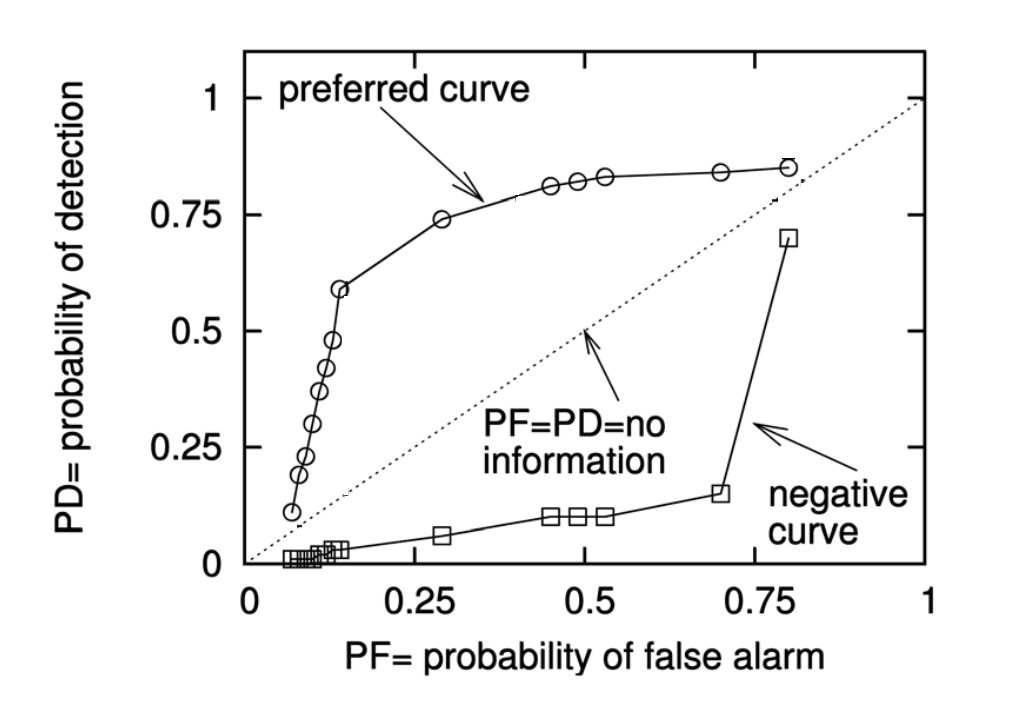
\includegraphics[width=.60\textwidth]{img/ROC.PNG}
	\caption{ نمونه‌ای از نمودار \lr{ROC} \cite{menzies2007data}}
	\label{fig:ROC}
\end{figure}

 مساحت زیر منحنی هزینه-اثربخشی معیاری است که تعداد خطوطی از برنامه که  توسط تیم تضمین کیفیت و یا توسعه‌دهندگان نیاز است بررسی و آزمون شود را در نظر می‌گیرد. منظور از بررسی بازبینی کد جهت یافتن خطا بدون استفاده از روش‌های مرسوم آزمون نرم‌افزار می‌باشد. ایده‌ی  موثر بودن از نظر هزینه
برای مدل‌های ‌‌ پیش‌بینی خطا برای اولین بار توسط آریشلم و همکاران \cite{arisholm2007data} ارائه گردید. موثر بودن از نظر هزینه به این معنا است که چه تعداد خطا با بررسی و یا آزمون  \lr{n}  درصد اول خطوط می‌توان یافت. به عبارت دیگر اگر یک مدل پیش‌بینی خطا بتواند تعداد خطای بیشتری را با بررسی و تلاش در آزمون کمتر، نسبت به باقی مدل‌ها بیابد می‌توان گفت که تاثیر آن از نظر هزینه بیشتر است. دو منحنی در  قسمت راست شکل \ref{fig:AUCEC} برای دو مدل پیش‌بینی مختلف آمده است. هر دو مدل دارای سطح زیر نمودار یکسانی هستند اما زمانی که ۲۰ درصد اول محور افقی در نظر گرفته می‌شود مدل 
\lr{P$_2$}
  کارایی بهتری دارد. نمودار سمت چپ مدل‌های تصادفی، عملی\LTRfootnote {Practical} و بهینه را نشان می‌دهد.

\begin{figure}[H]
	\centering
	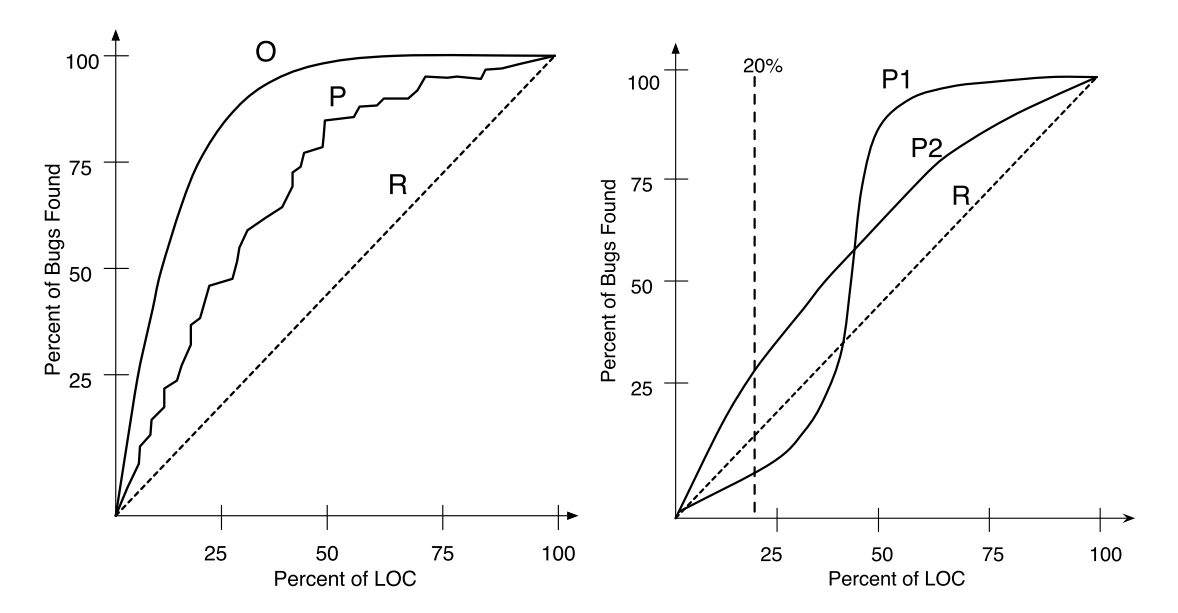
\includegraphics[width=.7\textwidth]{img/AUCEC.PNG}
	\begin{tabular}{c c c}
		\lr{O = optimal} & \lr{P = practical} &  \lr{R = random}\\
	 
	\end{tabular}
	\caption{ نمودار موثر بودن از نظر هزینه \cite{rahman2011bugcache}}
	\label{fig:AUCEC}
\end{figure}

معیارهایی که برای ارزیابی نتایج حاصل از روش رگرسیون به کار گرفته می‌شوند بر اساس همبستگی\LTRfootnote{Correlation} میان تعداد خطاهای پیش‌بینی شده و خطاهای واقعی محاسبه می‌شوند. نماینده‌ی این معیارها را می‌توان همبستگی اسپیرمن، پیرسون و $ R^2$ دانست \cite{nam2014survey}. 